% TeX шаблон, пример оформления отчёта по лабораторной работе.
% Автор: Шмаков И.А.
% Дата: 02 февраля 2018 года.
% Сборка документа из командной строки:
% ~$ pdflatex -shell-escape main.tex

\documentclass[a4paper,14pt]{extarticle}
\usepackage[utf8]{inputenc}
\usepackage[english,russian]{babel}
% Пакет отвечающий за рисование графиков в нутри TeX файла.
% https://ru.sharelatex.com/blog/2013/08/27/tikz-series-pt1.html
% https://ru.sharelatex.com/learn/TikZ_package
% http://tex.stackexchange.com/questions/300945/how-to-draw-this-picture-with-latex-tikz-pgf
\usepackage{tikz}

\usepackage{setspace}
\singlespacing % одинарный интервал

\usepackage{amsmath}
\usepackage{amsfonts}
\usepackage{amssymb}
\usepackage{mathtext}
\usepackage{graphicx}
\usepackage{float}
\usepackage[left=3cm, right=1cm, top=1.5cm, bottom=1.5cm]{geometry}
\usepackage{icomma} % "Умная" запятая: $0,2$ --- число, $0, 2$ --- перечисление
\usepackage{indentfirst} % Красная строка.
% Пакет отвечающий за листинги.
\usepackage{minted}
% Русский язык в листингах minted
% http://aakinshin.blogspot.ru/2014/01/latex-minted.html
% \makeatletter
% \newcommand{\minted@write@detok}[1]{%
%   \immediate\write\FV@OutFile{\detokenize{#1}}}%
% 
% \newcommand{\minted@FVB@VerbatimOut}[1]{%
%   \@bsphack
%   \begingroup
%     \FV@UseKeyValues
%     \FV@DefineWhiteSpace
%     \def\FV@Space{\space}%
%     \FV@DefineTabOut
%     %\def\FV@ProcessLine{\immediate\write\FV@OutFile}% %Old, non-Unicode version
%     \let\FV@ProcessLine\minted@write@detok %Patch for Unicode
%     \immediate\openout\FV@OutFile #1\relax
%     \let\FV@FontScanPrep\relax
% %% DG/SR modification begin - May. 18, 1998 (to avoid problems with ligatures)
%     \let\@noligs\relax
% %% DG/SR modification end
%     \FV@Scan}
%     \let\FVB@VerbatimOut\minted@FVB@VerbatimOut
% 
% \renewcommand\minted@savecode[1]{
%   \immediate\openout\minted@code\jobname.pyg
%   \immediate\write\minted@code{\expandafter\detokenize\expandafter{#1}}%
%   \immediate\closeout\minted@code}
% \makeatother
% Русский язык в листингах minted

\renewcommand{\thesection}{\arabic{section}}

% Описание титульной страницы
%\title{ГОУ ВО <<Алтайский государственный университет>>}
%\author{Шмаков И.А.}


\begin{document}
\begin{titlepage}
  \begin{center}
    ГОУ ВО АЛТАЙСКИЙ ГОСУДАРСТВЕННЫЙ УНИВЕРСИТЕТ
    \vspace{0.25cm}
    
    Физико-технический факультет
    
    Кафедра вычислительной техники и электроники
    \vfill
    
    {\LARGE Среды и средства разработки}\\[5mm]
    \textsc{(Отчёт по индивидуальному заданию по курсу <<Операционные системы>>)}
  \bigskip

\end{center}
\vfill

\newlength{\ML}
\settowidth{\ML}{«\underline{\hspace{0.7cm}}» \underline{\hspace{2cm}}}
\hfill\begin{minipage}{0.4\textwidth}
  Выполнил студент 2-го курса, 585 группы:\\
  \underline{\hspace{\ML}} А.\,К.~Роженцев\\
  «\underline{\hspace{0.7cm}}» \underline{\hspace{2cm}} \the\year~г.
\end{minipage}%
\bigskip

\hfill\begin{minipage}{0.4\textwidth}
  Проверил\\
  \underline{\hspace{\ML}} П.\,Н.~Уланов\\
  «\underline{\hspace{0.7cm}}» \underline{\hspace{2cm}} \the\year~г.
\end{minipage}%
\vfill

\begin{center}
  Барнаул, \the\year~г.
\end{center}
\end{titlepage}

%\maketitle

\tableofcontents

\section{Введение и постановка задачи}
Требуется написать программу, на вход которой поступает четыре значения (A, B, C, D), операции между операндами
требуется получить у преподавателя. Примечание: сборка исполнимого файла должна осуществляться через GNU make.

\section{Приложение}
\begin{minted}[mathescape,linenos,frame=lines]{C}
#include "moncar.h"

int main()
{
        double A,B,C,D;
        double result=0;
        A = 10;
        B = 15;
        C = 20;
        D = 25;
        result = A / B - C * D;
        printf("result=%lf\n",result);
        return 0;
}
\end{minted}
\section{Содержание Makefile}
\begin{minted}[mathescape,linenos,frame=lines]{make}
#default target - file edit
default: link
link: main_moncar.o
	cc -o main main_moncar.o
main_moncar.o: main_moncar.c moncar.h
	cc -c main_moncar.c
clean:
	rm main main_moncar.o
\end{minted}



%\section{Алгоритм и блок-схема}
%В данном пункте отчёта требуется предоставить алгоритм работы программы и блок-схему, 
%а также информацию о правилах в соответствии с которыми были построены алгоритм и 
%блок-схема.

%\section{Проверка работы программы}
%В данном пункте отчёта требуется предоставить данные по работе программы. В частности
%сравнение ваших результатов для какой-либо приближенной функции и <<оригинальной>> функции.
%\begin{figure}[H]
%\centering 
%\begin{tikzpicture}
%\draw (0,0) parabola (5,5);
%\draw (0,0) .. controls (0,4) and (4,0) .. (4,5);
%\draw[step=1cm,gray,very thin] (-1.5,-1.5) grid (5.9,5.9);
%\draw[thick,->] (0,0) -- (5.5,0) node[anchor=north west] {x};
%\draw[thick,->] (0,0) -- (0,5.5) node[anchor=south east] {y};
%
%\foreach \x in {0,1,2,3,4,5}
%    \draw (\x cm,1pt) -- (\x cm,-1pt) node[anchor=north] {$\x$};
%\foreach \y in {0,1,2,3,4,5}
%    \draw (1pt,\y cm) -- (-1pt,\y cm) node[anchor=east] {$\y$};
%    
%\end{tikzpicture}
%\caption{Пример использования Tikz} 
%\end{figure}


\section{Вывод по работе}
\begin{figure}[h!]
\centering
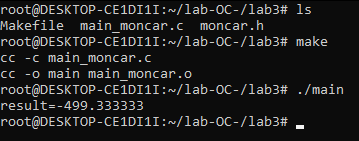
\includegraphics[width=1\linewidth]{vivod.png}
\caption{Вывод}
\label{fig:mpr}
\end{figure}


%\renewcommand\bibname{Список литературы}
%\addcontentsline{toc}{section}{Список литературы}
%\begin{thebibliography}{99}
%\bibitem{catheydow} W.T. Cathey and E.R. Dowski, <<New paradigm for imaging systems>>, Appl. Opt. 41, pp. 6080-6092, 2002.
%\end{thebibliography}

%\addcontentsline{toc}{section}{Приложение}
%\section*{Приложение}
%\begin{minted}[mathescape,linenos,frame=lines]{python}
%import numpy as np
% 
%def incmatrix(genl1,genl2):
%    m = len(genl1)
%    n = len(genl2)
%    M = None #to become the incidence matrix
%    VT = np.zeros((n*m,1), int)  #dummy variable
% 
%    #compute the bitwise xor matrix
%    M1 = bitxormatrix(genl1)
%    M2 = np.triu(bitxormatrix(genl2),1) 
% 
%    for i in range(m-1):
%        for j in range(i+1, m):
%            [r,c] = np.where(M2 == M1[i,j])
%            for k in range(len(r)):
%                VT[(i)*n + r[k]] = 1;
%                VT[(i)*n + c[k]] = 1;
%                VT[(j)*n + r[k]] = 1;
%                VT[(j)*n + c[k]] = 1;
% 
%                if M is None:
%                    M = np.copy(VT)
%                else:
%                    M = np.concatenate((M, VT), 1)
% 
%                VT = np.zeros((n*m,1), int)
% 
%    return M
%\end{minted}
%
%\begin{minted}[mathescape,linenos,frame=lines]{C}
%#include "stdio.h"
%
%int main(){
%  int a, b, c; 
%  
%  a = 5;
%  b = 10;
%  c = a + b;
%  
%  printf("Результат сложения a + b = %i\n", c);
%  
%  return 0;
%}
%\end{minted}


\end{document} 